\documentclass[14pt]{beamer}

\usepackage{amssymb,amsfonts,amsmath,mathtext}
\usepackage{cite,enumerate,float,indentfirst}

\graphicspath{{../images/}{images/}} 

\usepackage{../Dissertation/phdstyle}
\usepackage[edges]{forest}
\usepackage{tcolorbox}
\newcommand{\ntrn}{n_{turn}}
\newcommand{\gef}{\gamma_{eff}}
\renewcommand{\ecm}{$e\cdot$cm}

\newcommand{\wedm}{\w^{edm}}
\newcommand{\wmdm}{\w^{mdm}}
\newcommand{\wimp}{\w^{imp}}

\title[Thesis presentation]{Frozen spin method of search for the deuteron EDM in a storage ring}
\author[A. Aksentev]{Alexander Aksentev \inst{1,2}}
\institute[NRNU MEPhI]{
	\inst{1} Forschungszentrum J\"ulich \and%
	\inst{2} NRNU ``MEPhI''
}
\date{18 July 2019}

\usetheme{Boadilla}

\begin{document}
	\maketitle
	
	
\section{Formal setup}
\begin{frame}{Research goal and objectives}
	\textbf{Goal:} to evaluate the proposed method's capability to detect the deuteron EDM at the sensitivity level $10^{-29}$\ecm \\
	\pause
	\textbf{Objectives:}
	\begin{itemize}
		\item effect of betatron oscillations on the validity of the EDM statistic
		\item spin-decoherence near zero resonance
		\item properties of the MDM faking signal due to machine imperfections
		\item the calibration and exclusion of the faking signal from the EDM static
		\item evaluation of statistical sensitivity
	\end{itemize}
\end{frame}

\begin{frame}{Claims to be defended}
	\begin{itemize}[<+->]
		\item The frequency domain method's EDM statistic is robust with regard to perturbations from the particles' betatron motion
		\item The machine imperfections faking signal's properties
		\begin{itemize}
			\item necessitate the use of a frequency domain method of search for the EDM
			\item make it possible to exclude this signal from the target statistic
		\end{itemize}
	\end{itemize}
\end{frame}
\begin{frame}{Claims to be defended}
	\begin{itemize}[<+->]
		\item Spin tune can be expressed as a function of a \textbf{single} parameter (effective Lorentz factor), which is a measure of the particle's longitudinal emittance
		\item The effective Lorentz factor is susceptible to calibration
		\item It is statistically possible to reach a standard error of the mean EDM estimate at the level $10^{-29}$\ecm~in year's worth of beam time
	\end{itemize}
\end{frame}

\section{Space vs frequency domain approaches}
\begin{frame}{Space vs frequency domain methods}
	$P_y = A\cdot \sin\bkt{\underbrace{\sqrt{(\wedm + \wimp)^2 + \w_y^2 + \w_z^2}}_{\W}\cdot t + \delta}$
	\begin{itemize}
		\item \textbf{Space domain:}
		\begin{itemize}
			\item (Must!) Stop MDM precession in the \textbf{vertical}, as well as \textbf{horizontal}, plane
			\item Track the change in spatial orientation of the polarization vector
		\end{itemize}
		\item \textbf{Frequency domain:}
		\begin{itemize}
			\item Stop \textbf{only} the horizontal plane precession
			\item Track the change in the vertical plane precession angular velocity
		\end{itemize}
	\end{itemize}
\end{frame}

\begin{frame}{What are the advantages of frequency domain?}
	\begin{enumerate}
		\item Element alignment specifications aren't as severe
		\item Stable spin wheel state solves the geometric phase error problem
		\item Easier polarimetry
	\end{enumerate}
\end{frame}

\section{Main part}
\subsection{Betatron motion effect}
\begin{frame}{Betatron motion effect}
	\begin{block}{EDM statistic}
		$\hat\wedm = \frac12 (\hat\w_x^+ + \hat\w_x^-)$, where $\w_x^\pm = \wedm \pm\wmdm$
	\end{block}
	\begin{block}{Frequency estimated via fit}
		$f(t) = a\cdot\sin(\w_x\cdot t + \delta)\mapsto \hat\w_x$, where $(a, \w_x, \delta) = \const$
	\end{block}
	\begin{block}{While the solution of T-BMT}
		$a = \sqrt{\nbar_x^2 + (\nbar_y\cdot \nbar_z)^2}$, where $\nbar = g(\vec E, \vec B)$
	\end{block}
\end{frame}

\begin{frame}\frametitle{Simulation}\centering
	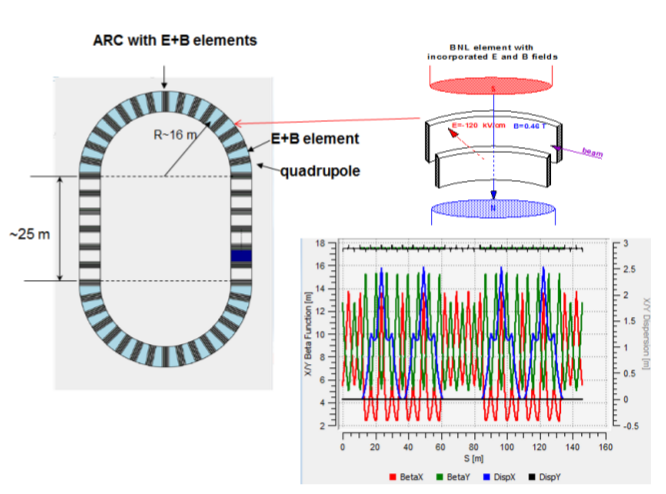
\includegraphics[width=.8\linewidth]{chapter2/BNL_lattice}
\end{frame}
\begin{frame}\frametitle{Simulation}
	\begin{minipage}[t]{.48\linewidth}
	\textbf{Machine\\ imperfections}
	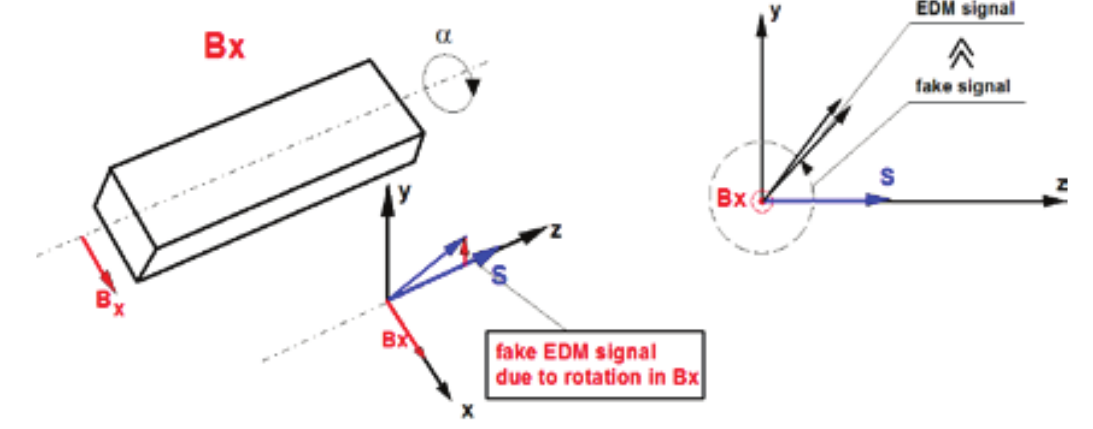
\includegraphics[width=1.2\linewidth, trim=80 10 0 0, clip]{images/magnet_tilting}
	\begin{itemize}
		\item $\alpha\sim N(\mu_i, 3\cdot10^{-4})^\circ$
		\item $\mu_i$ simulates the application of a spin wheel driver
	\end{itemize}
	\end{minipage}~~~~
	\begin{minipage}[t]{.45\linewidth}
	\textbf{Particles}
	\begin{itemize}
		\item betatron oscillating in the vertical plane
		\item $E_{FS}\neq E_{kin}\to E_{FS}$
		\item[$\Rightarrow$] $\nbar_x\ll 1 \Rightarrow$ high sensitivity to perturbations
	\end{itemize}
	\end{minipage}
\end{frame}
\begin{frame}\frametitle{Analysis}
	\begin{minipage}[t]{.5\linewidth}
		\textbf{Data}
		\begin{itemize}
			\item[TRK] data from the COSY Infinity tracker
			\item[GEN] computed from the fit function, with $\nbar$, $\nu_s$ from tracking
			\item[IDL] as in GEN, but $\nbar = \avg{\nbar}$, $\nu_s = \avg{\nu_s}$ 
		\end{itemize}
	\end{minipage}~~~~
	\begin{minipage}[t]{.5\linewidth}
		\textbf{Comparator\\ stats}
		\begin{itemize}
			\item[$\epsilon_1(t)$] $= s_y^{gen}(t) - s_y^{idl}(t)$
			\item[$\epsilon_2(t)$] $= s_y^{trk}(t) - s_y^{idl}(t)$
		\end{itemize}
	\end{minipage}
\end{frame}
\begin{frame}\frametitle{Results}
	\begin{tikzpicture}
		\node (resid) {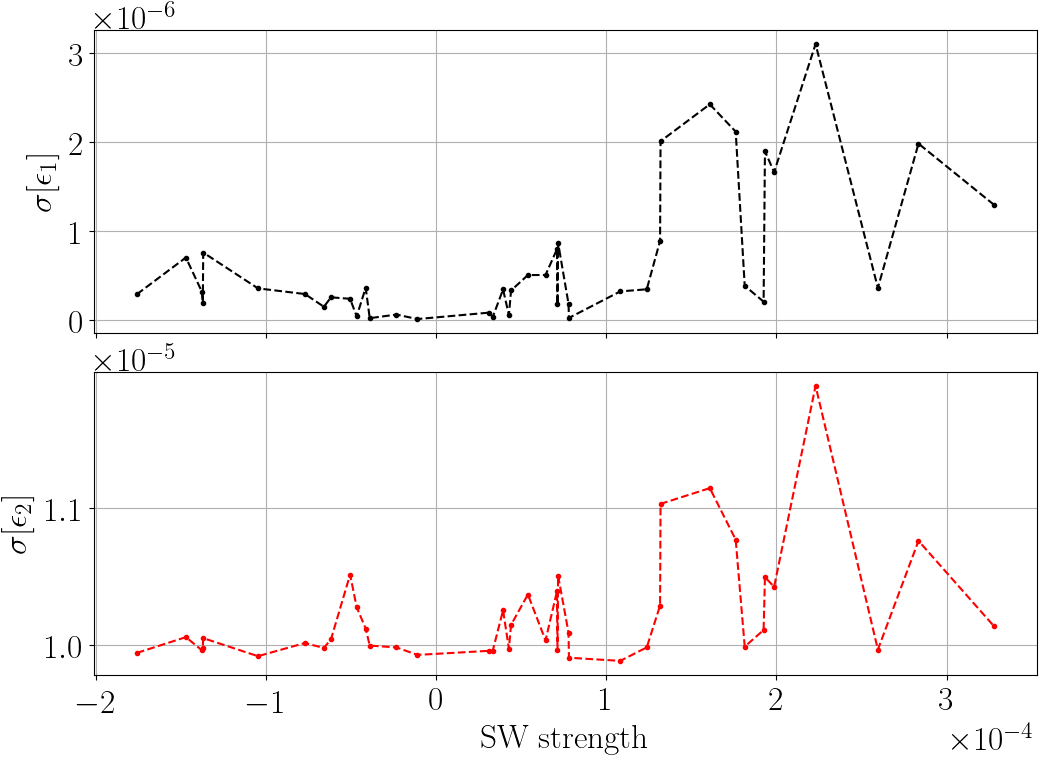
\includegraphics[width=.7\linewidth]{smp_sim/residual_SD_vs_SW(both)}};
		\pause
		\node (nbar) at (resid.center)[xshift=2.5cm,yshift=-2cm]{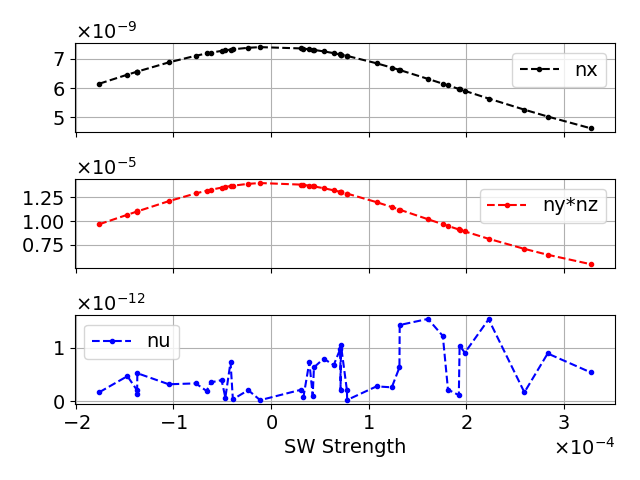
\includegraphics[width=.7\linewidth]{smp_sim/NBAR_variation_sd_vs_SW}};
	\end{tikzpicture}	
\end{frame}
\begin{frame}\frametitle{Conclusions}
	\begin{enumerate}[<+->]
		\item The signal amplitude oscillations (as estimated by $\epsilon_2$) are small.
		They occur at the level at least two orders of magnitude smaller than the expected polarization measurement error. This means the superposition of this systematic error with the random measurement error
		will exhibit no statistically-significant systematicity.
	\end{enumerate}
\end{frame}
\begin{frame}{Conclusions}
	\begin{enumerate}\setcounter{enumi}{1}
		\item The correllation coefficient between the amplitude and frequency estimates is not significant. The amplitude oscillations affect the $\hat a$-estimate foremost; their effect on the $\hat\w$-estimate is secondary, and is described by the correlation coefficient. Since it is less than 10\%, even if the oscillations happen to be
		strong enough to affect the amplitude estimate, their effect on the frequency estimate will be reduced by
		at least a factor of 10.
	\end{enumerate}
\end{frame}
\begin{frame}{Conclusions}
	\begin{enumerate}
		\setcounter{enumi}{2}
		\item This systematic effect is controllable. And this point is the major advantage of the FD methodology.
		By applying an external Spin Wheel, the $\nbar$ oscillations can be continuously minimized
		as much as necessary, without changing the pattern of the experiment.
	\end{enumerate}
\end{frame}

\subsection{Spin decoherence}
\begin{frame}{Spin decoherence}
	\framesubtitle{Cause}
	\begin{minipage}{.65\linewidth}
		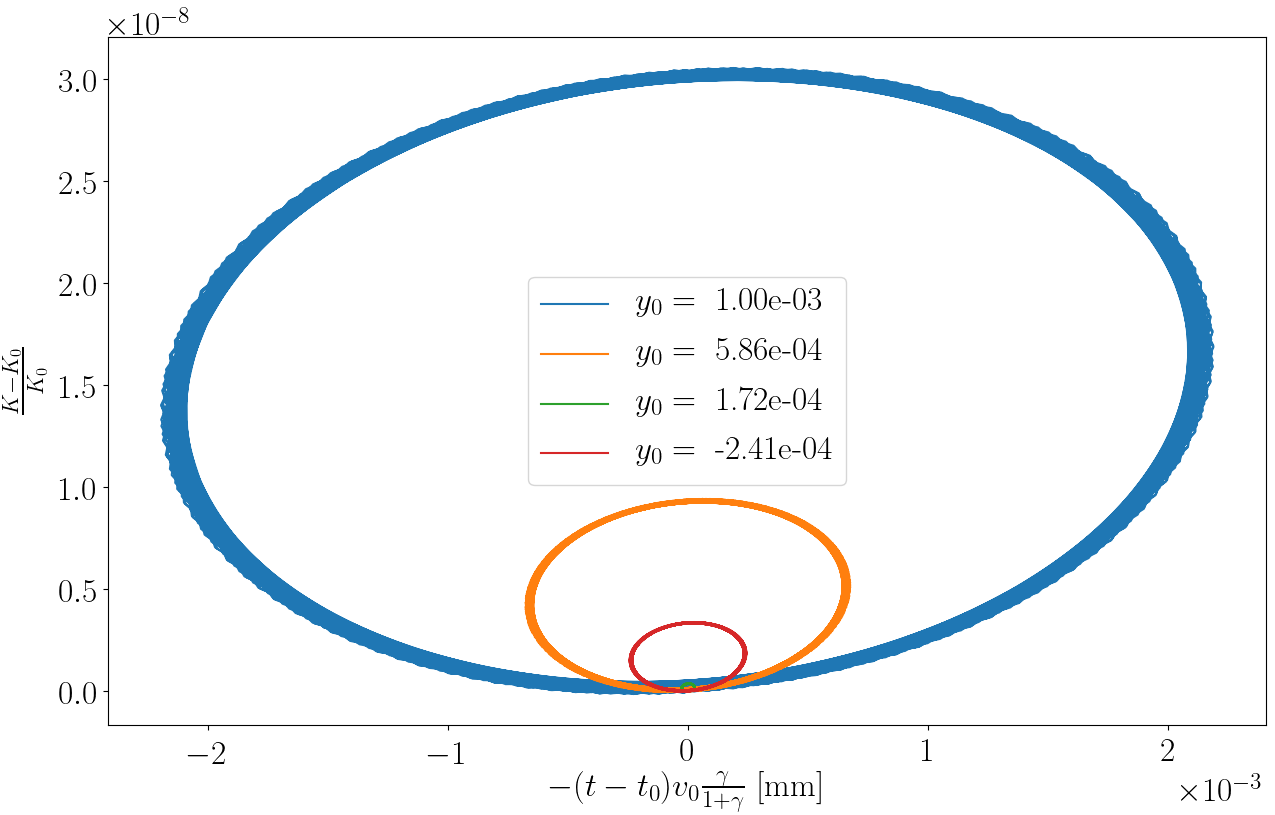
\includegraphics[width=\linewidth]{chapter1/psp_diagram_betatron}
	\end{minipage}%
	\begin{minipage}{.4\linewidth}
		\begin{itemize}
			\item $\nu_s = \gamma G$
			\item because of the orbit length difference, beam particles have different $\gamma_{eq}$ 
		\end{itemize}
	\end{minipage}
\end{frame}
\begin{frame}{Supression via sextupole field}
	\begin{block}{Equilibrium level momentum shift}
		$\Delta\delta_{eq} = \frac{\gamma_0^2}{\gamma_0^2\alpha_0 - 1}\bkt*{\frac{\delta_m^2}{2}\bkt{\alpha_1 - \alpha_0\gamma^{-2} + \gamma_0^{-4}} + \bkt{\frac{\Delta L}{L}}_\beta}$
	\end{block}
	\begin{block}{Sextupole field effects}
		\begin{forest}
			forked edges,
			for tree={edge={->},  rounded corners, grow'=0}
			[{$S_{sext} = \frac{1}{B\rho} \pddx{B_y}[x][2]$}
			[{$\Delta \alpha_{1,sext} = -\frac{S_{sext}D_0^3}{L}$}]
			[{$\bkt{\frac{\Delta L}{L}}_{sext} = \mp \frac{S_{sext}D_0\beta_{x,y}\varepsilon_{x,y}}{L}$}]
			]
		\end{forest}
	\end{block}
\end{frame}
\begin{frame}{Sextupole field effects}
	\framesubtitle{Momentum compaction factor}
	\begin{tikzpicture}
		\node (main) {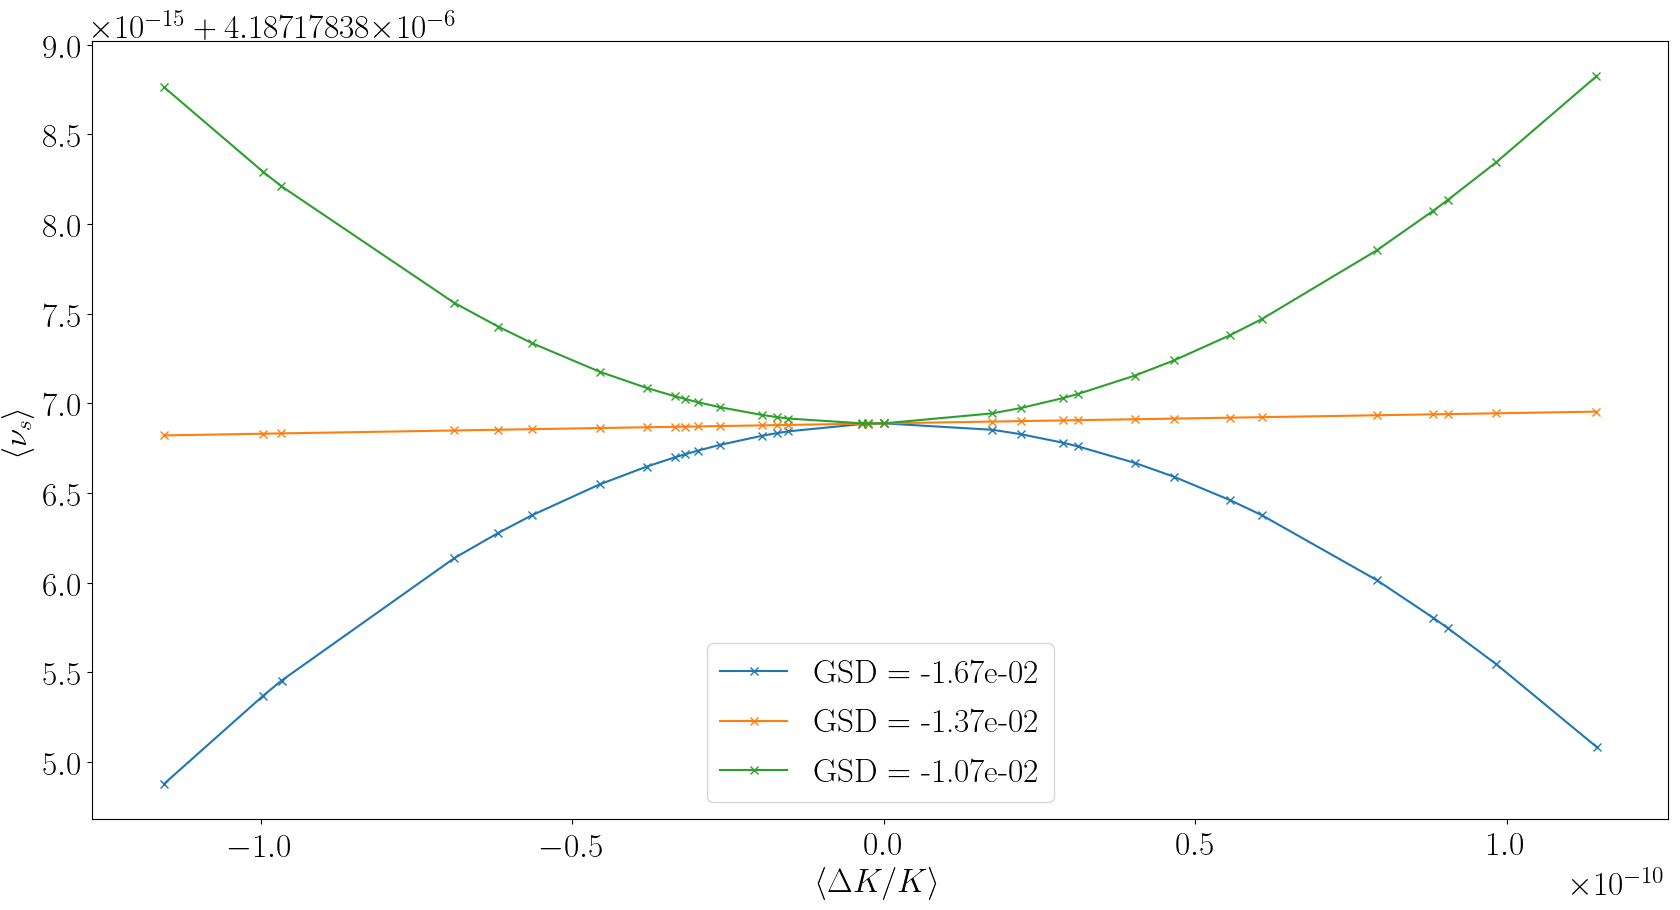
\includegraphics[width=.7\linewidth]{decoh_sim/propdef/stune_vs_dkok_SS_D}};
		\pause
		\node (PS) at (main.east)[yshift=-2cm, xshift=-.8cm] {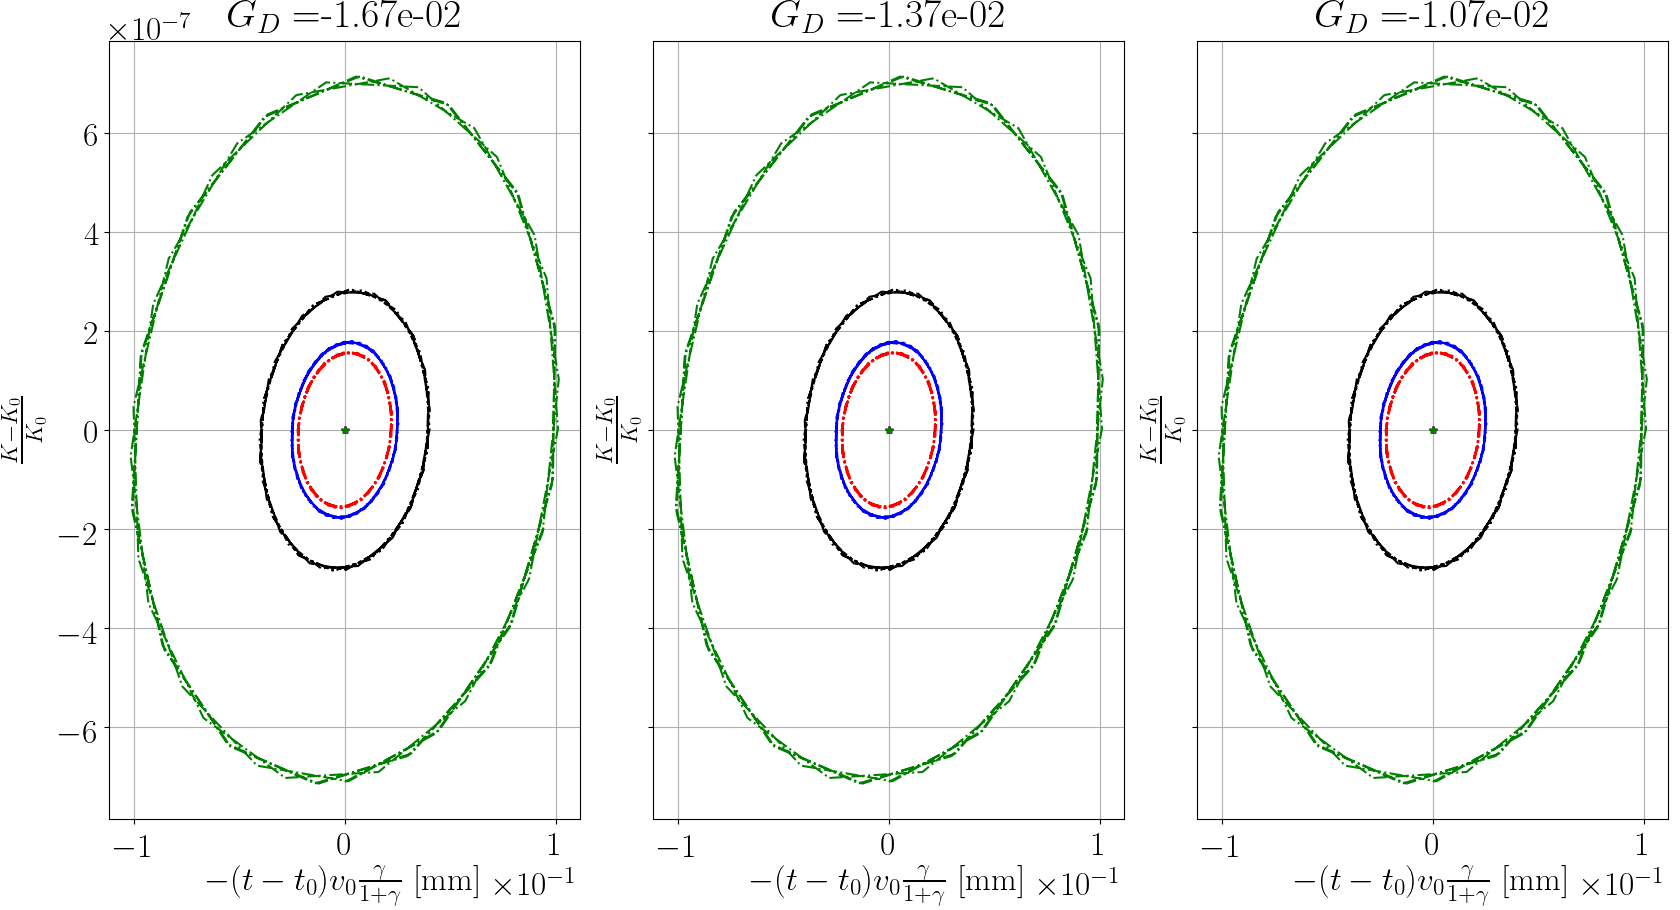
\includegraphics[width=.7\linewidth]{decoh_sim/propdef/long_phase_space_for_sext_settings_D}};
	\end{tikzpicture}
\end{frame}
\begin{frame}{Sextupole field effects}
	\framesubtitle{Orbit length}
	\begin{tikzpicture}
		\node (main) {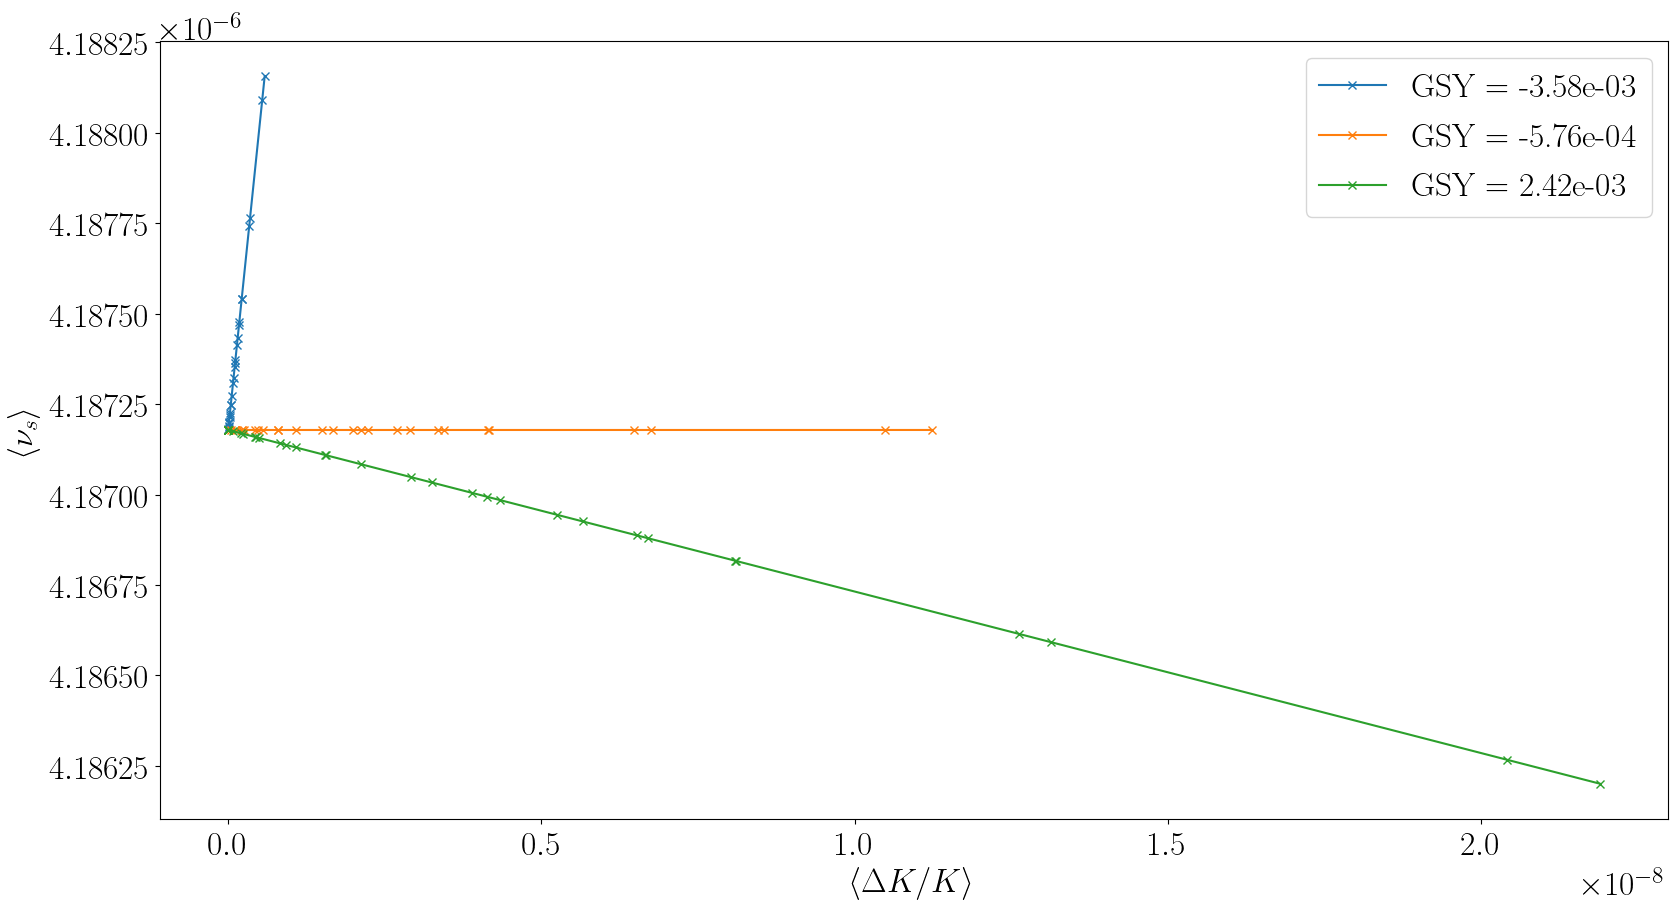
\includegraphics[width=.7\linewidth]{decoh_sim/propdef/stune_vs_dkok_SS_Y}};
		\pause
		\node (PS) at (main.east)[yshift=-2cm, xshift=-.8cm] {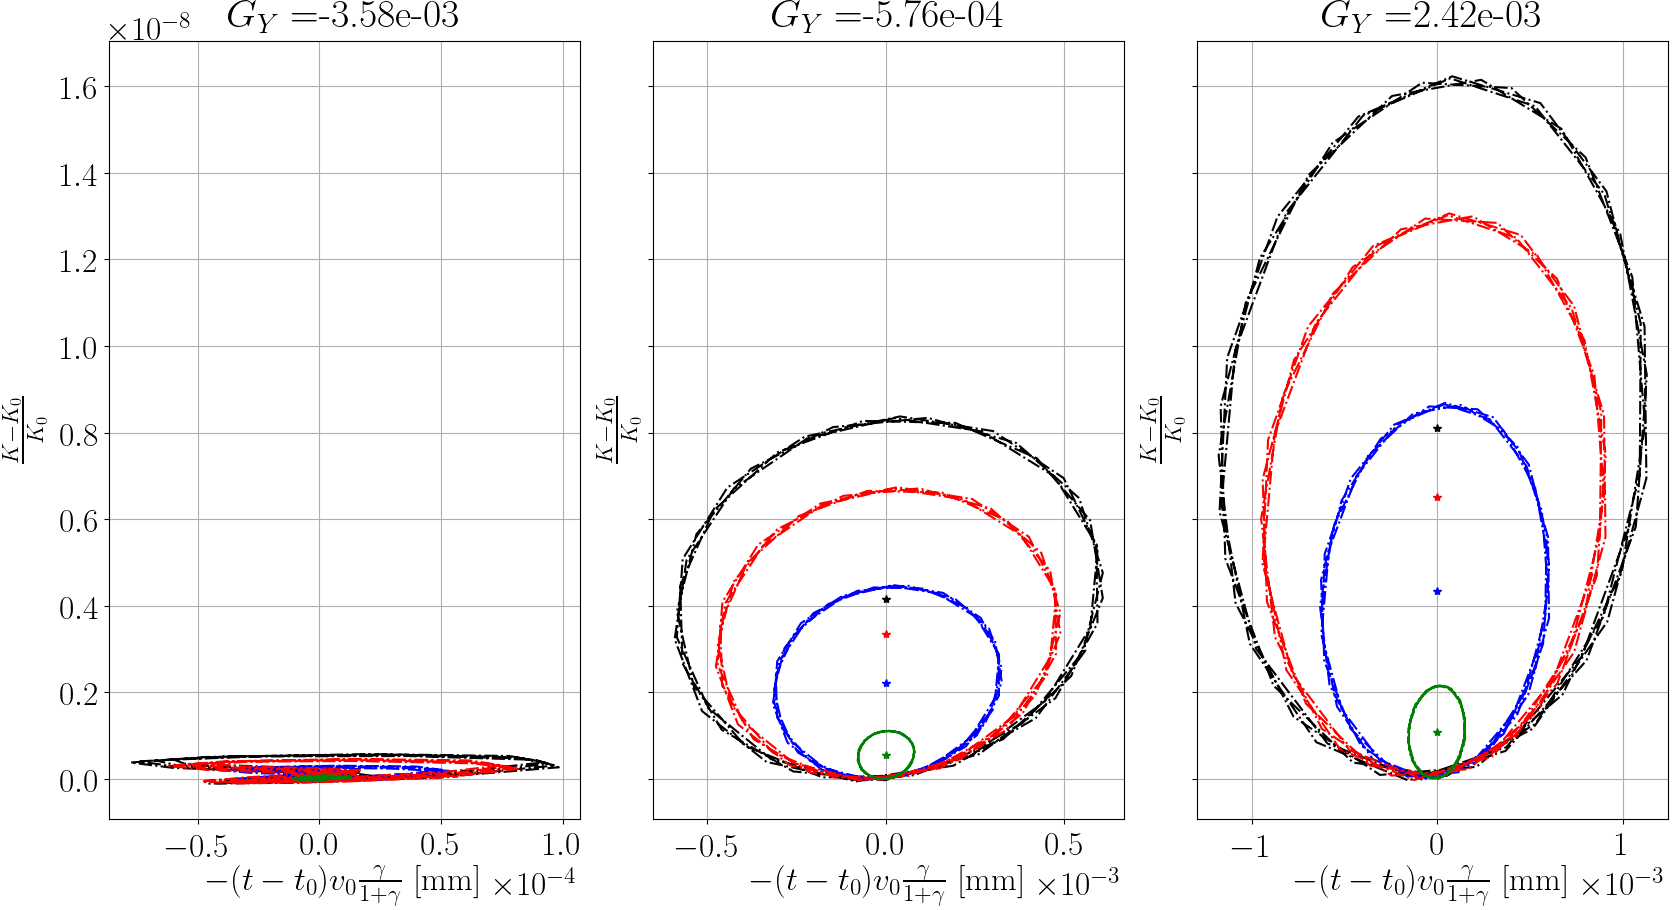
\includegraphics[width=.7\linewidth]{decoh_sim/propdef/long_phase_space_for_sext_settings_Y}};
	\end{tikzpicture}
\end{frame}

\begin{frame}{Conclusions}
	\begin{enumerate}[<+->]
		\item The signature of the sextupole field's momentum compaction effect is the change in the functional form of $\avg{\nu_s}(\avg{\Delta K/K})$
		\item \ldots~ orbit length effect --- reduction in the dispersion of $\avg{\Delta K/K}$
	\end{enumerate}
\end{frame}

\begin{frame}{Decoherence supression in an ideal lattice}\centering
	\begin{tikzpicture}
		\node (X) {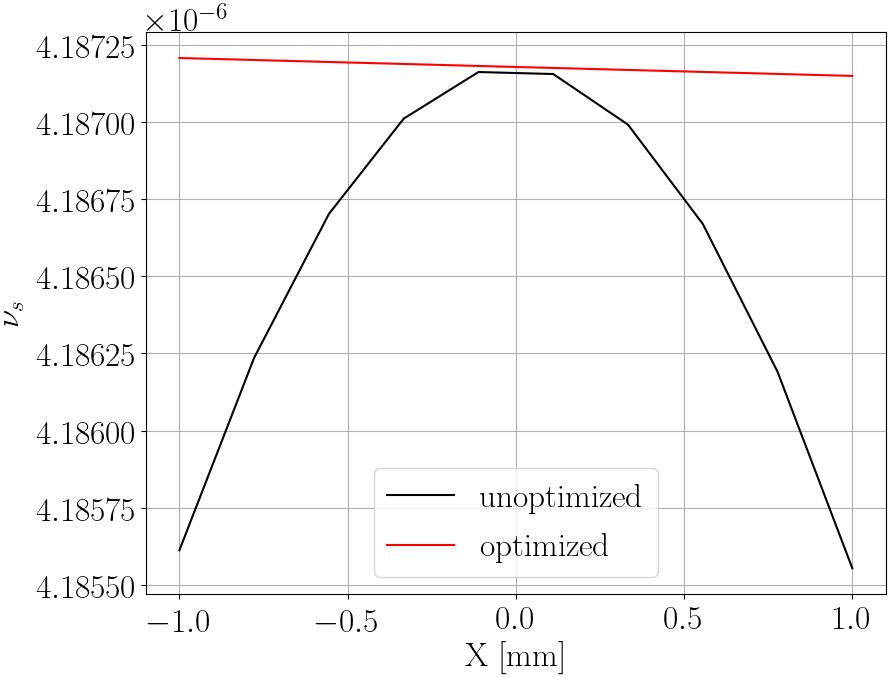
\includegraphics[height=.5\paperheight]{decoh_sim/spin_tune_decoh_x_offset}};
		\pause
		\node (Y) at (X.east)[yshift=-1.7cm]{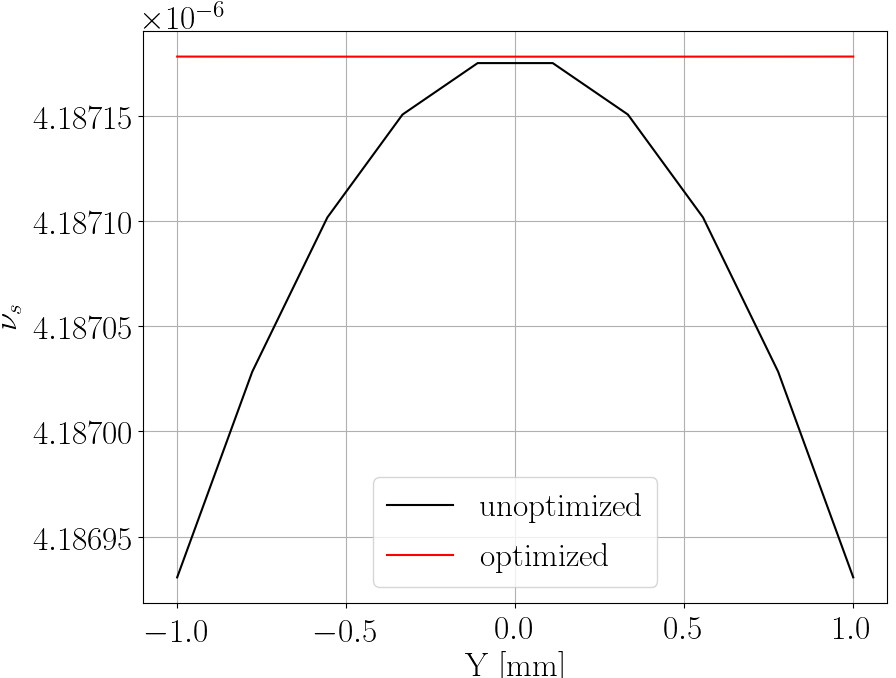
\includegraphics[height=.5\paperheight]{decoh_sim/spin_tune_decoh_y_offset}};
		\pause
		\node (D) at (X.center)[yshift=-2.3cm]{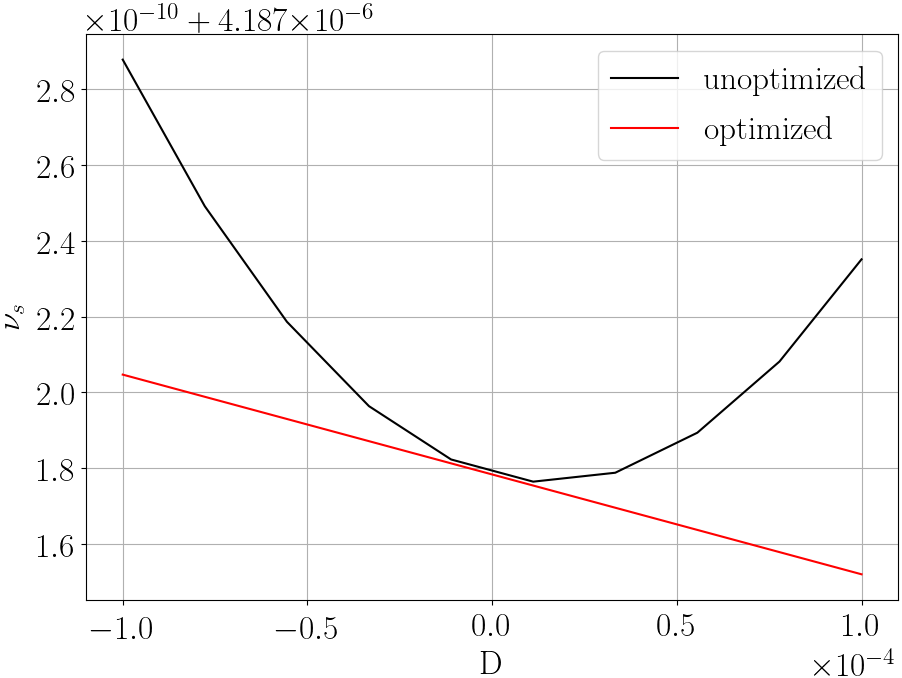
\includegraphics[height=.5\paperheight]{decoh_sim/spin_tune_decoh_d_offset}};
	\end{tikzpicture}
\end{frame}
\begin{frame}{Decoherence in an imperfect lattice}
	\begin{tikzpicture}
		\node (imgX) {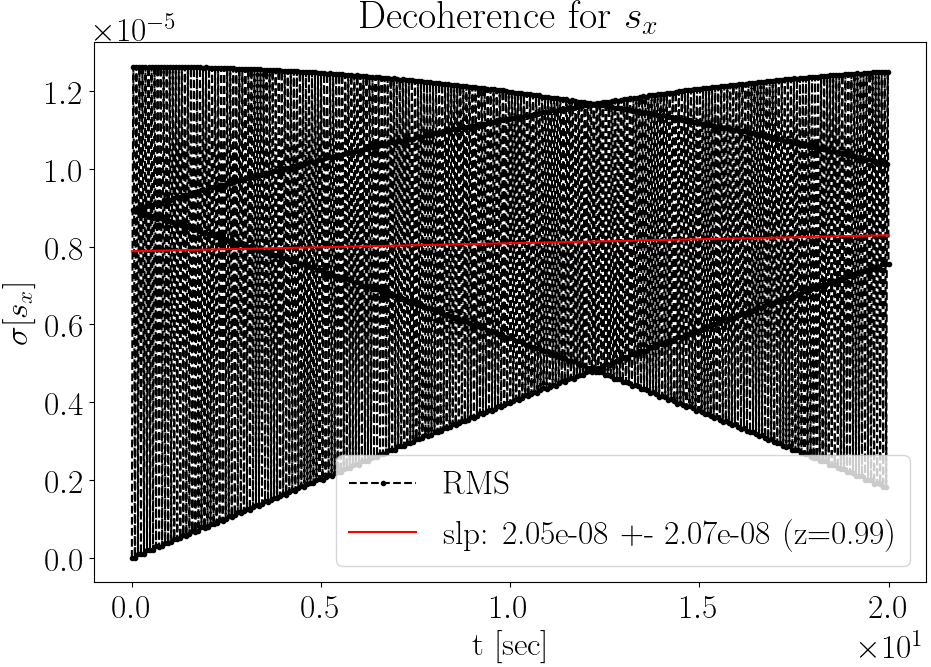
\includegraphics[width=.65\linewidth]{decoh_sim/SX_decoh_20sec_unopt}};
		\pause
		\node (imgY) at (imgX.south east)[yshift=1cm]{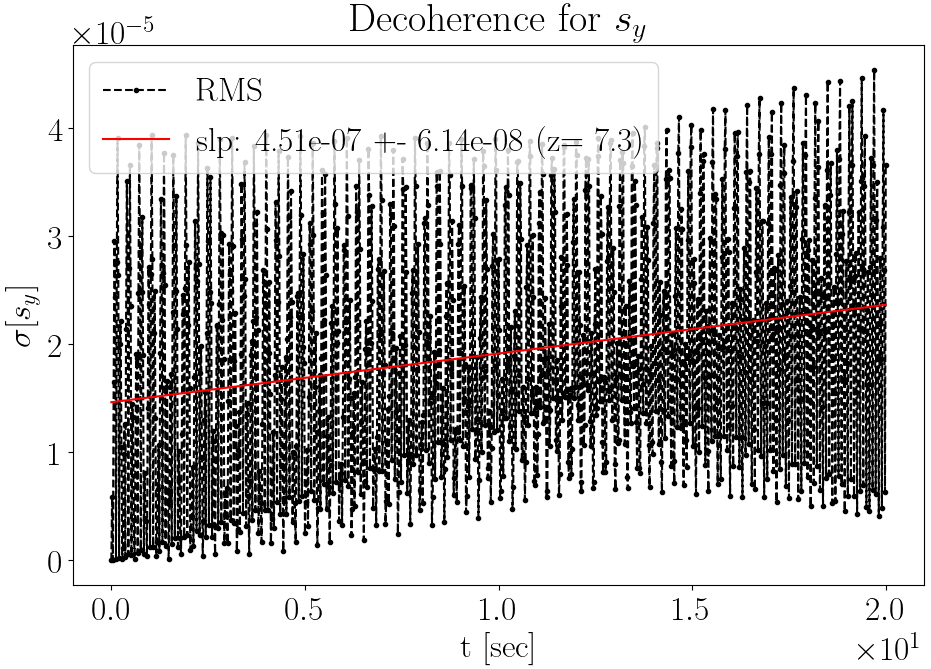
\includegraphics[width=.65\linewidth]{decoh_sim/SY_decoh_20sec_unopt}};
	\end{tikzpicture}
\end{frame}
\begin{frame}{Turning on the sextupoles}
	\begin{tikzpicture}
		\node (imgX) {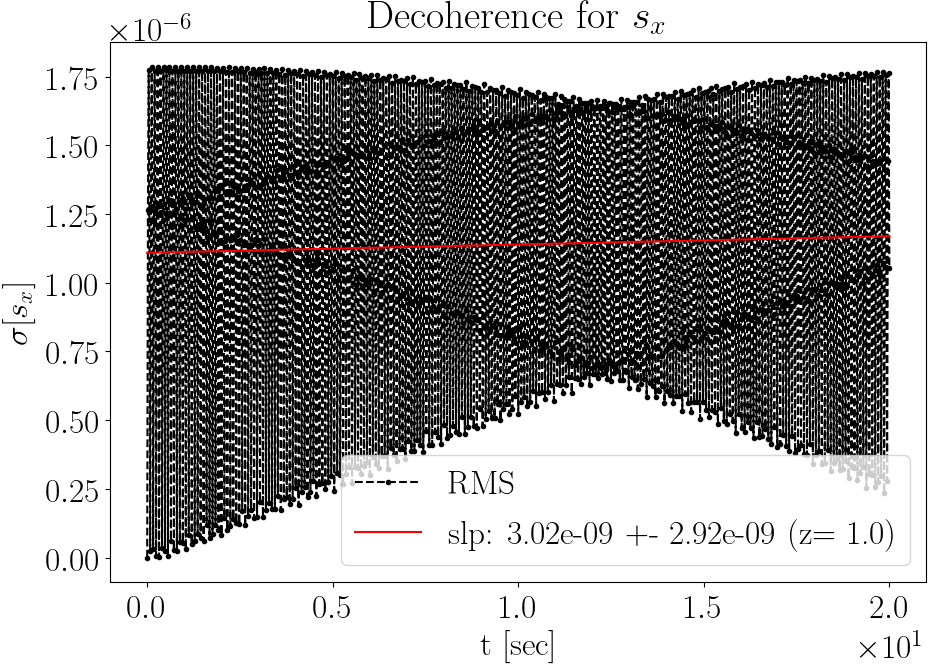
\includegraphics[width=.65\linewidth]{decoh_sim/SX_decoh_20sec_opt}};
		\pause
		\node (imgY) at (imgX.south east)[yshift=1cm]{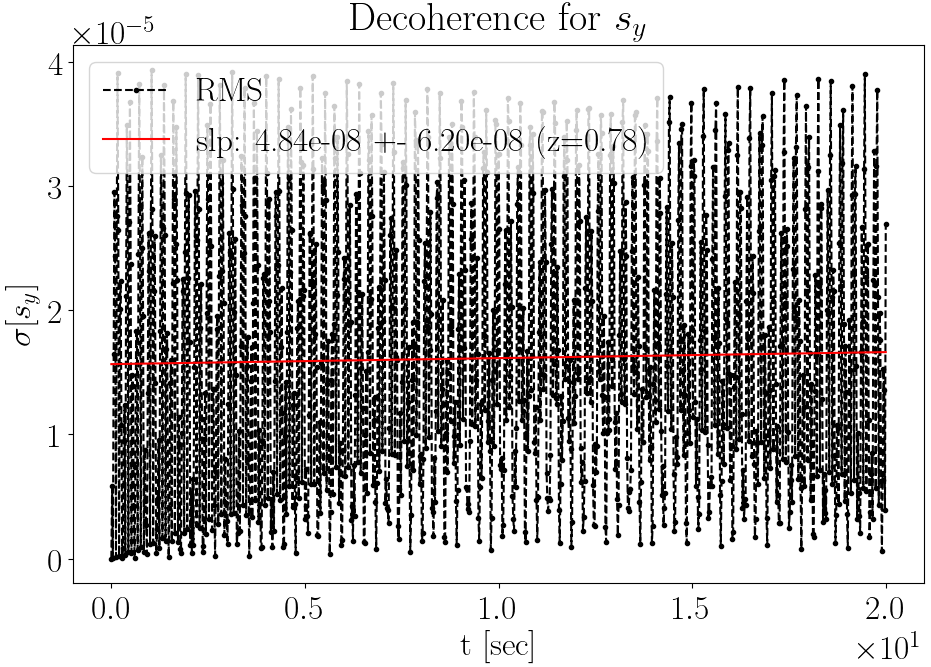
\includegraphics[width=.65\linewidth]{decoh_sim/SY_decoh_20sec_opt}};
	\end{tikzpicture}
\end{frame}

\subsection{Faking signal}
\begin{frame}{MDM faking signal}
	\begin{block}{Magnitude}
		$\SD{\W_x^{MDM}} = \frac{q}{m\gamma}\frac{G+1}{\gamma}\frac{\SD{B_x}}{\sqrt{n}}$
	\end{block}
	\begin{block}{Questions to consider}
		\begin{itemize}
			\item Is the error linear, i.e. $\W_x^{MDM} = f(\avg{\Theta_{tilt}})$?
			\item Is it symmetric with regard to the beam circulation direction change, i.e. $|\W_x^{CW}| = |\W_x^{CCW}|$?
		\end{itemize}
	\end{block}
\end{frame}
\begin{frame}{Analyzed lattice}
	\begin{tikzpicture}
		\node (lat) {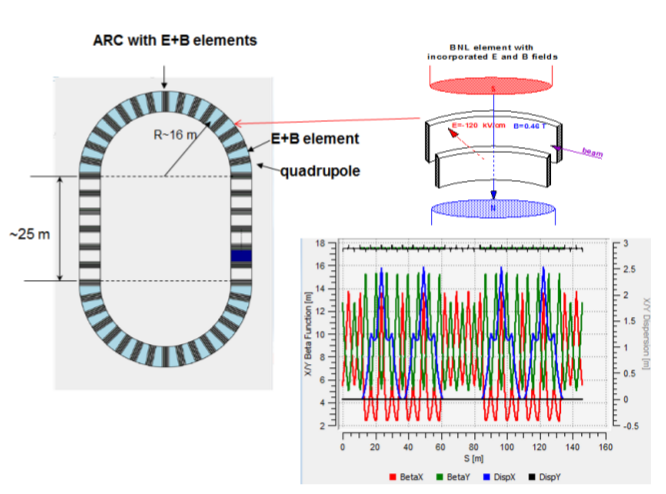
\includegraphics[width=.8\linewidth]{chapter2/BNL_lattice}};
		\pause
		\node (tilt) at (lat.center)[xshift=2cm,yshift=-1.6cm] {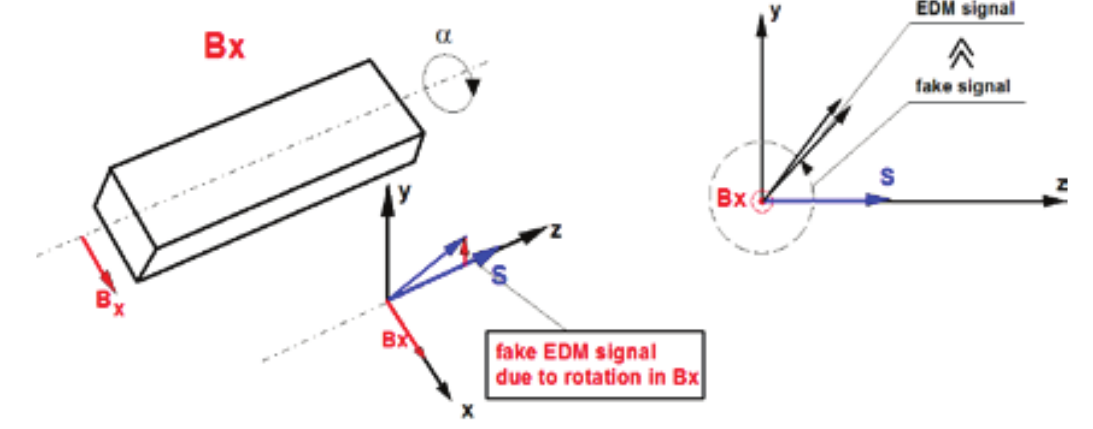
\includegraphics[width=.77\linewidth,trim = 30 0 0 0, clip]{images/magnet_tilting}};
		\pause
		\node (sim) at (lat.center)[xshift=-2cm, yshift=2cm] {
		\begin{tcolorbox}[width=.6\linewidth]
			\begin{minipage}{\linewidth}
				\begin{itemize}
					\item 11 simulations
					\item tilted only E+Bs
					\item $\alpha\sim N(\mu_0\cdot(i-5), \sigma_0)$
					\item $\mu_0 = 10\cdot\sigma_0 = 10^{-4}$ rad
					\item Taylor up to 3rd order
					\item computed $\W_x^{CO}$
				\end{itemize}
			\end{minipage}
		\end{tcolorbox}
		};
	\end{tikzpicture}
\end{frame}
\begin{frame}{Linearity}\centering
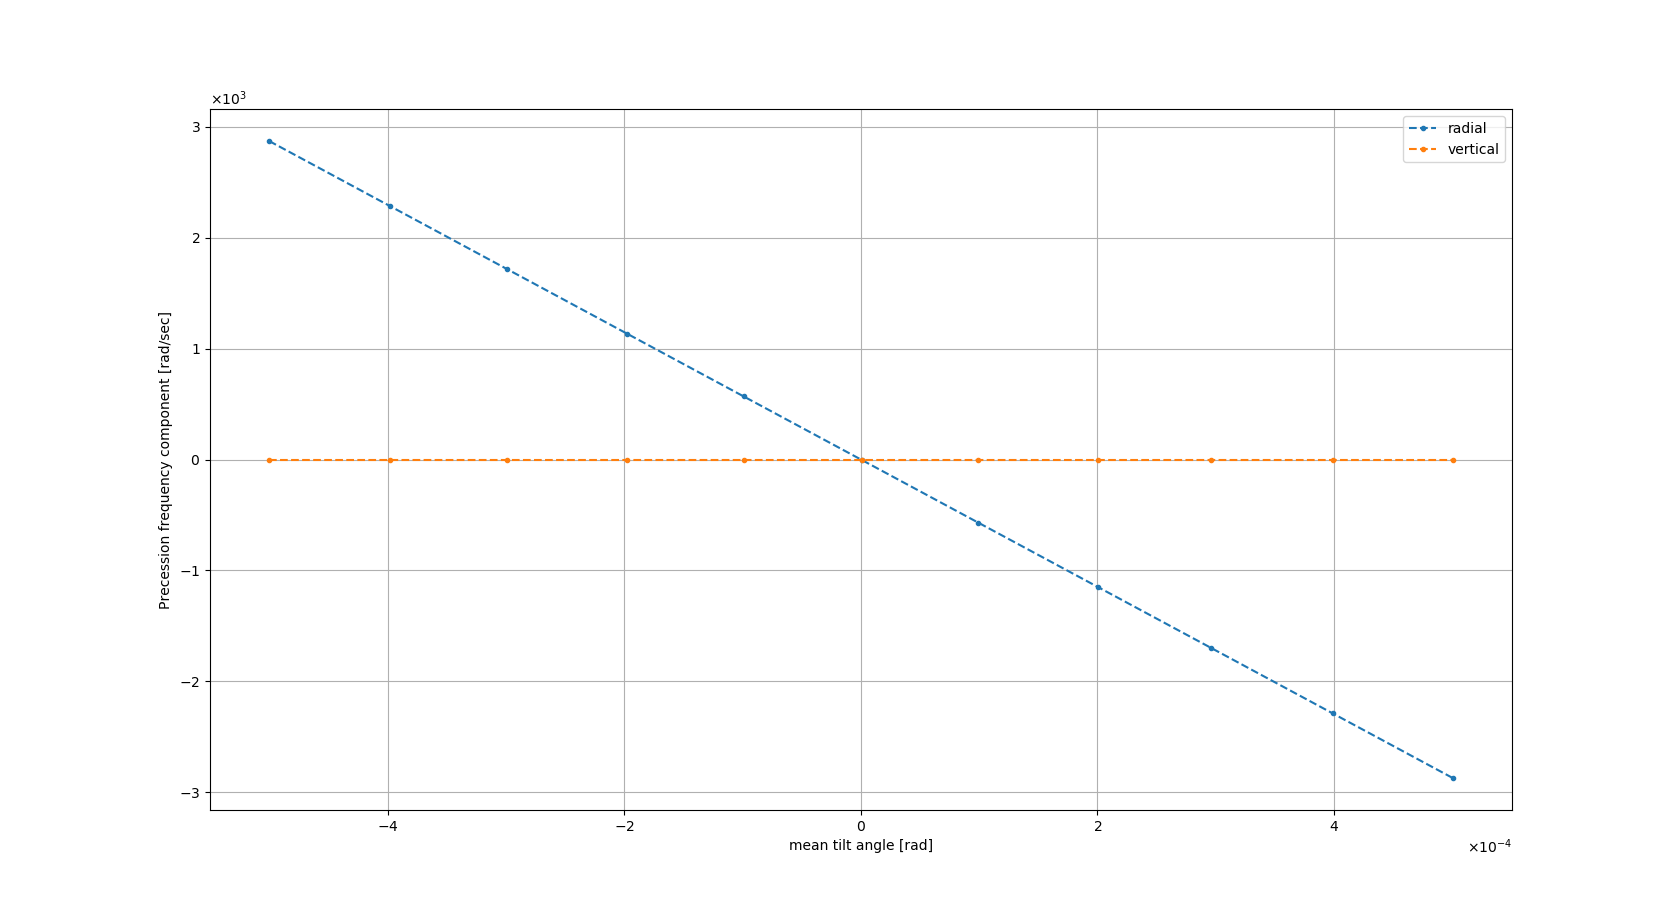
\includegraphics[width=.8\linewidth]{fake_signal_sim/linearity_test_shifting_gauss_freq}
\end{frame}
\begin{frame}{Symmetricity}
	\hspace*{-.9cm}
	\begin{tikzpicture}
		\node (first) {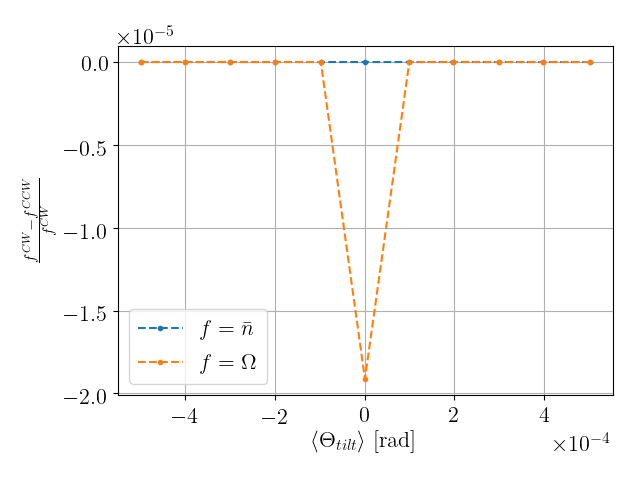
\includegraphics[width=.8\linewidth]{fake_signal_sim/linearity_test_shifting_gauss_rel_diff}};
		\pause
		\node (second) at (first.center)[xshift=2.5cm,yshift=-1.3cm] {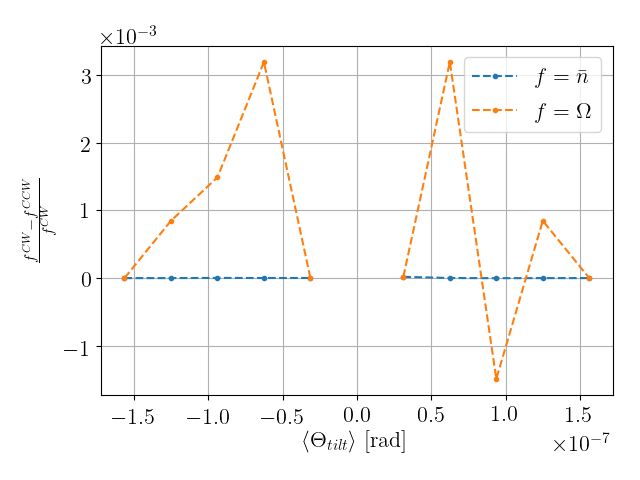
\includegraphics[width=.8\linewidth]{fake_signal_sim/linearity_test_compensated+microrad_rel_diff}};
	\end{tikzpicture}
\end{frame}
\begin{frame}{Conclusions}
	\begin{block}{$\sigma_\theta = 10^{-4}$ rad, $n=100$ elements}
		\begin{tabular}{r|r}
			\hline
			$\w^{max}$ [rad/sec] & $P(\W_x^{MDM} < \w^{max})$\\
			\hline
			50  & 67\%\\
			100 & 95\%\\
			\hline
		\end{tabular}
	\end{block}
	\begin{block}{Properties}
		\begin{enumerate}
			\item Linearity
			\item Asymmetricity, likely due to the difference between the CW and CCW beams' closed orbits
			\item Asymmetricity is less pronounced at higher SW roll rates
		\end{enumerate}
	\end{block}
\end{frame}

\subsection{Calibration procedure}
\begin{frame}{Guide field polarity reversal}
	\framesubtitle{Why?}\centering
	\begin{tikzpicture}
		\node (null) {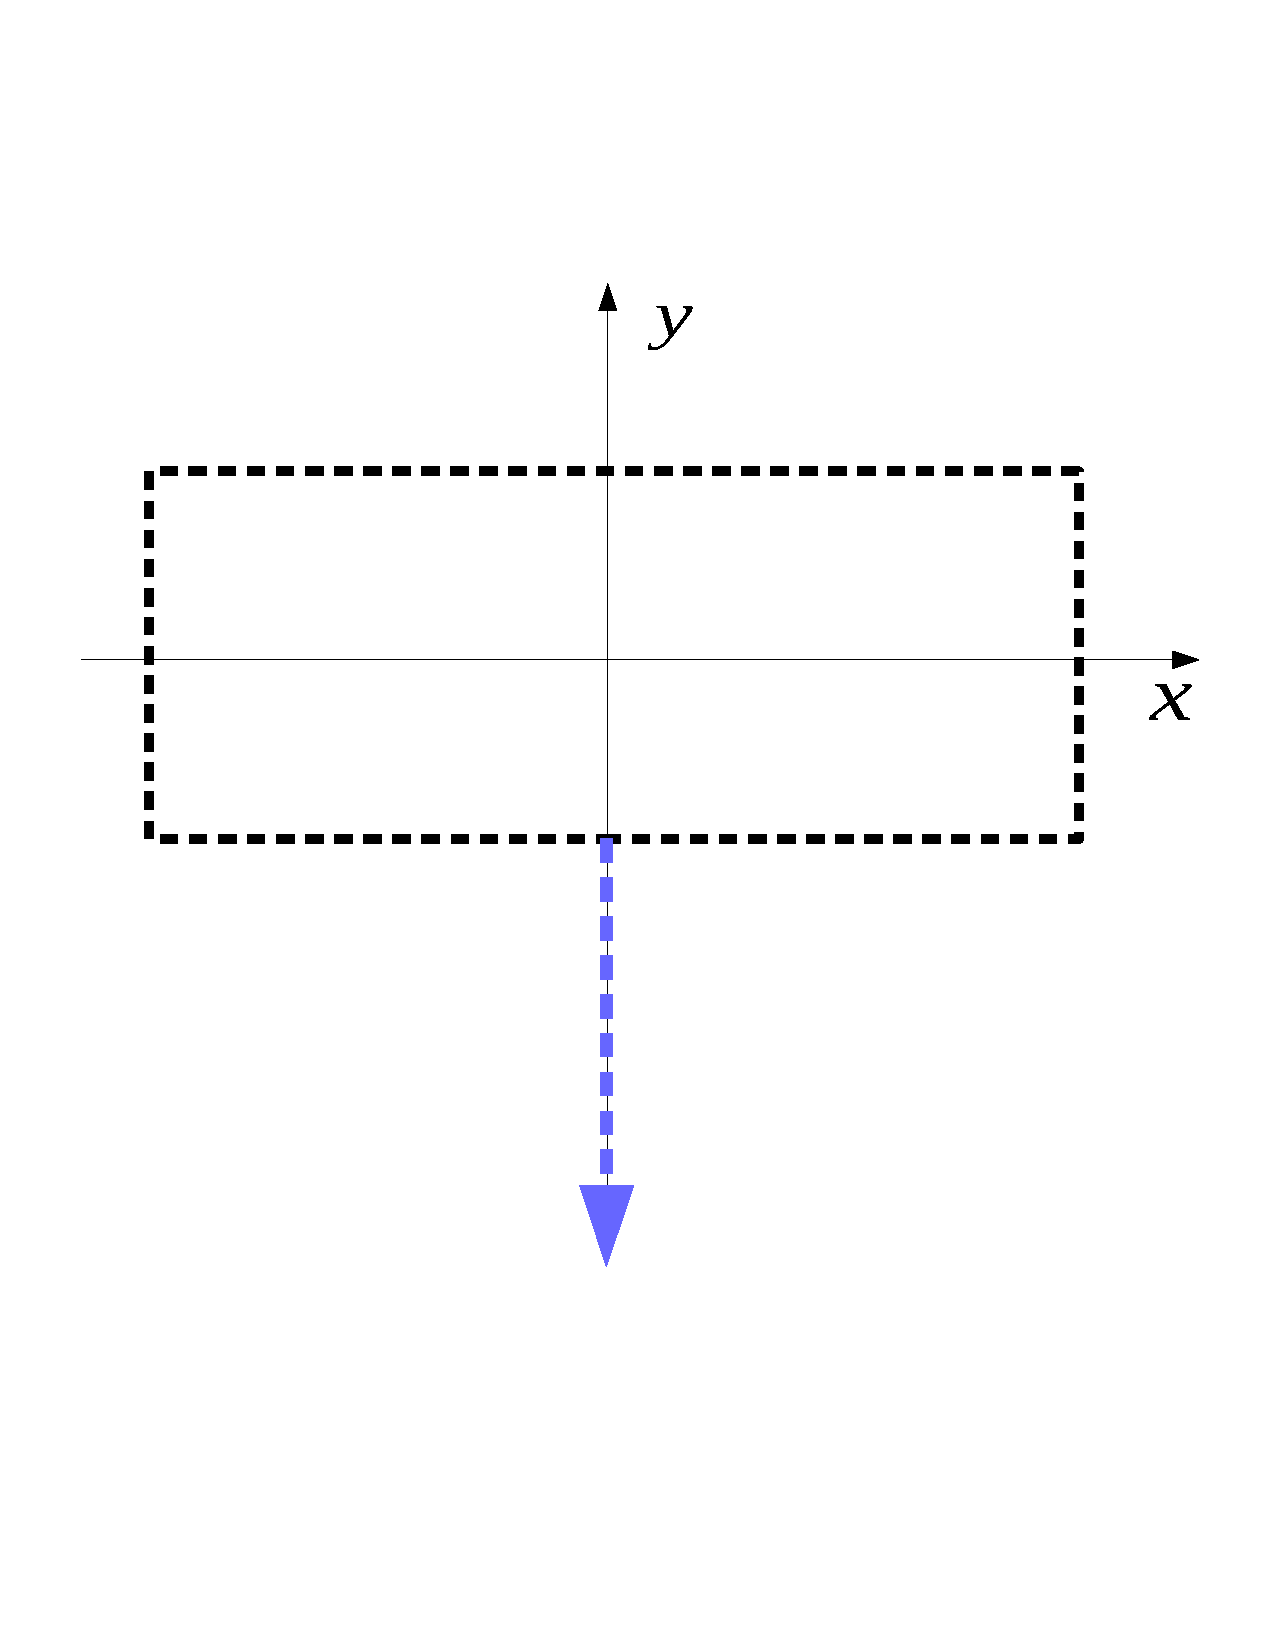
\includegraphics[height=.7\paperheight, trim=5 145 0 135, clip]{images/magnet_tilted-0.pdf}};
		\foreach \i in {1,...,3}
		{
			\pause
			\node (\i) at (null.center) {\includegraphics[height=.7\paperheight, trim=5 145 0 135, clip]{images/magnet_tilted-\i.pdf}};
		}
		\node (eq) at (null.south east)[yshift=.4cm] {$\hat\W_{edm} = \frac12\bkt{\W_x^{CW} + \W_x^{CCW}}$};
	\end{tikzpicture}
\end{frame}
\begin{frame}{Wherein lies the problem?}
	\begin{itemize}[<+->]
		\item $\W_x^{MDM} = \frac qmGB_x$
		\item Really, what needs to be reproduced is $\W_x^{MDM}$, \textbf{not} $B_x$
		\item Reproducing $B_x^{CW} = -B_x^{CCW}$ is not sufficient, because the beam injection point, and hence $\nu_s$, vary from cycle to cycle
		\item Besides, one has the lattice's spin dynamics asymmetry to consider (above)
		\item[$\Rightarrow$] Must reproduce the beam's effective Lorentz factor
	\end{itemize}
\end{frame}
\begin{frame}{Calibration of the effective L-factor}
	\begin{itemize}[<+->]
	\item $\nu_s$ is an injective function of $\gef$, meaning $\W_y(\gef^1) = \W_y(\gef^2) \to \gef^1=\gef^2$
	\item The particle orbit space can be partitioned into equivalence classes $[\gef]$
	\item[$\Rightarrow$] $\exists!\gef^0$: $[\gef^0] = [\W_y=0]$
	\item[$\Rightarrow$] if both CW, CCW beams are ``frozen'' in the horizontal plane, their $\gef$ are equal
	\end{itemize}
\end{frame}
\begin{frame}{Simulation}
	\begin{tikzpicture}
		\node (pic) {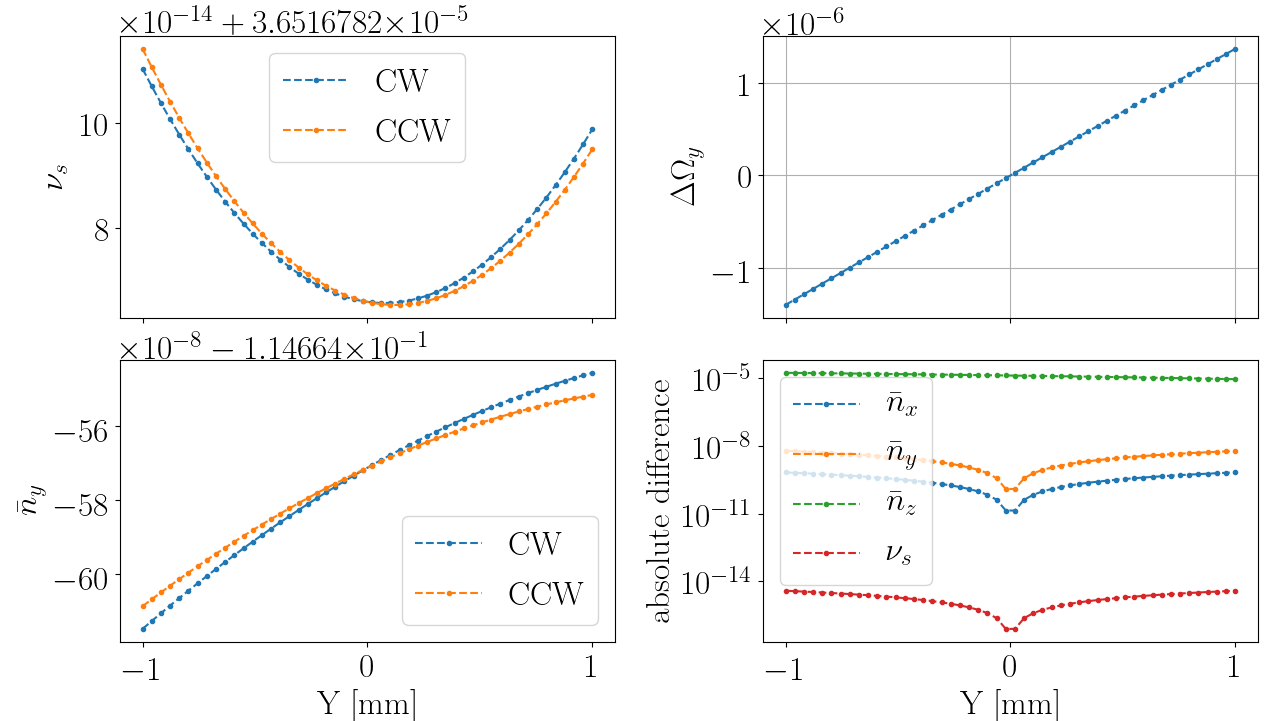
\includegraphics[width=\linewidth]{GFF/GFF_stune_range_Y}};
		\pause
		\node (expl) at (pic.center)[xshift=3.1cm, yshift=2.1cm] {
		\begin{tcolorbox}[height=3.6cm,width=.5\linewidth]
			\begin{minipage}{\linewidth}
				\begin{itemize}
					\item Same $S_{sext}$ works for both beams
					\item $\nu_s^{CW} \approx \nu_s^{CCW} \Rightarrow |\W_x^{CW}| \approx |\W_x^{CCW}|$
				\end{itemize}
			\end{minipage}
		\end{tcolorbox}
		};
		\pause
		\node (calib) at (expl.south)[yshift=-1.8cm] {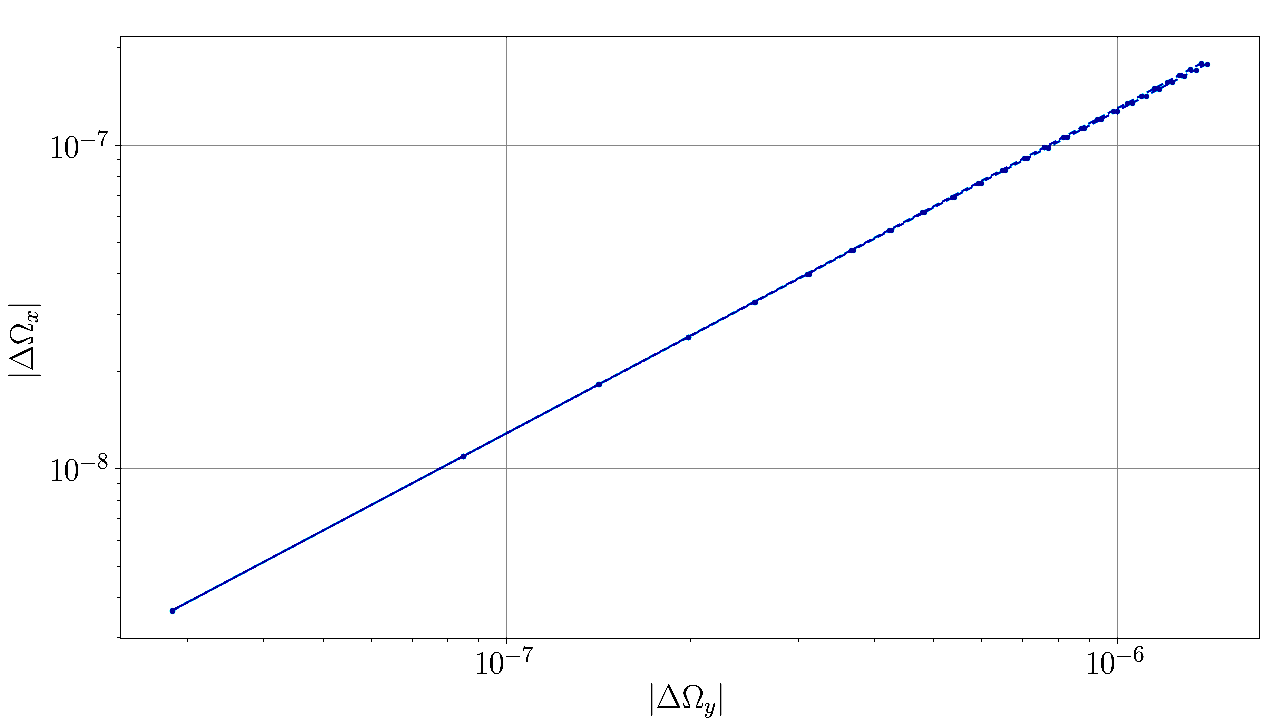
\includegraphics[width=.52\linewidth]{GFF/GFF_omegas_range_Y}};
	\end{tikzpicture}
\end{frame}

\subsection{Effective L-factor}
\begin{frame}{Spin tune a univariate function}
	\hspace*{-2cm}
	\begin{tikzpicture}
		\node (emiT) {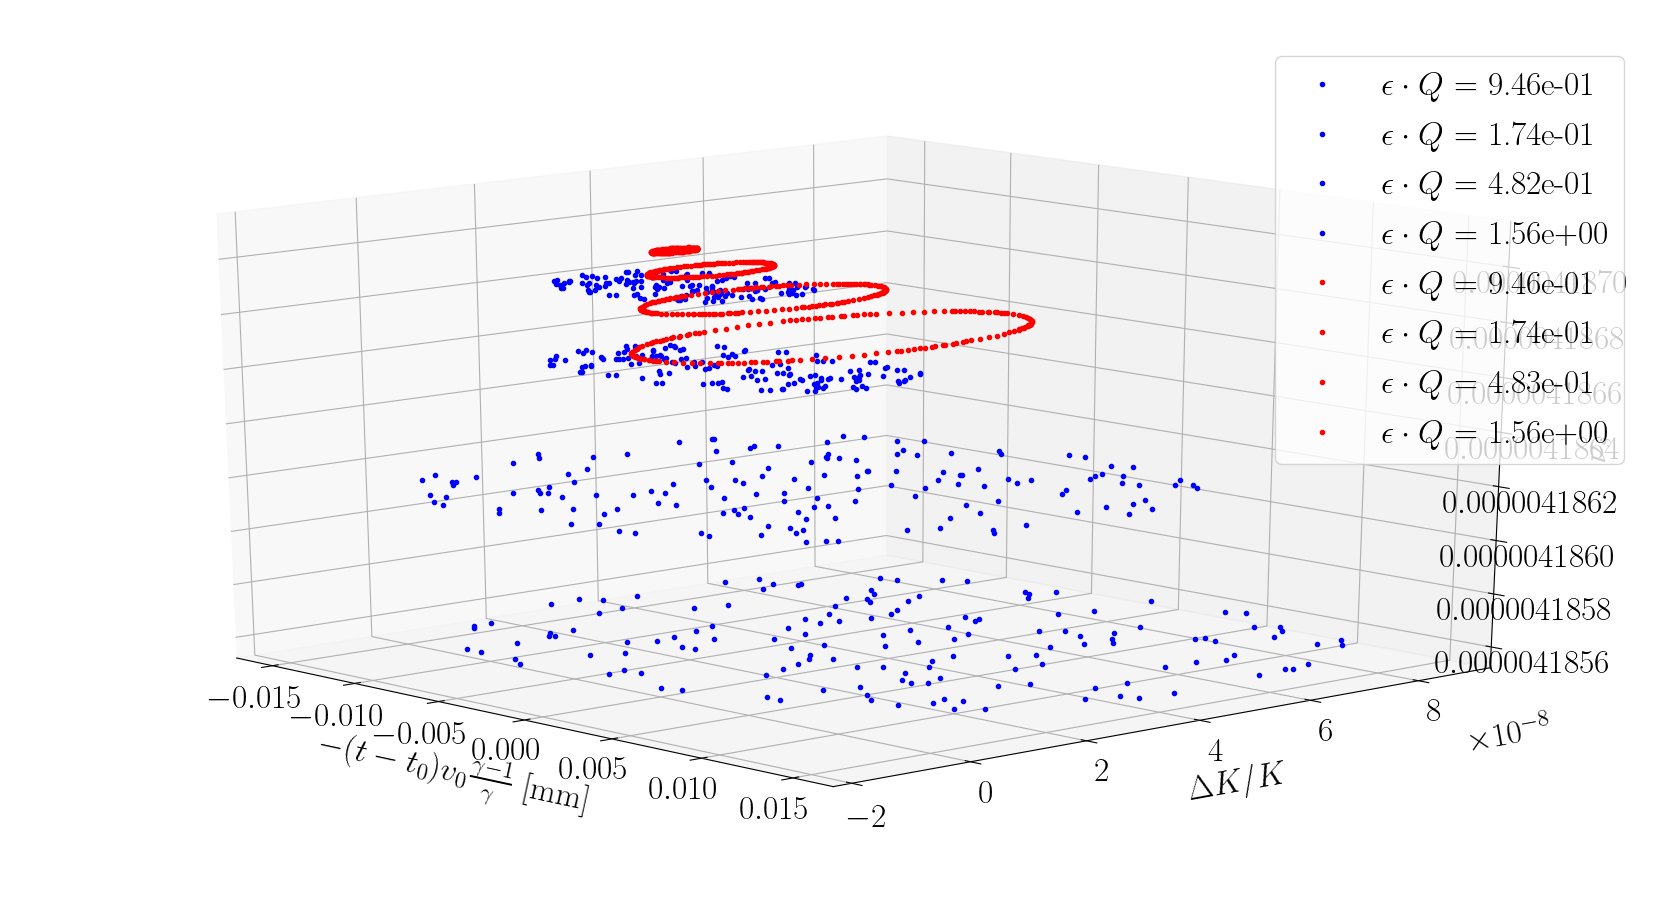
\includegraphics[width=.9\linewidth]{stune_traj_equ/part2/3D_plot_all_ps_vars}};
%		\pause
%		\node (emiQ) at (emiT.north)[yshift=1cm]{
%			\begin{tcolorbox}[width=.75\linewidth]
%			\small{
%				$\gef \propto \bkt*{\frac{\delta_m^2}{2}\bkt{\alpha_1 - \alpha_0\gamma^{-2} + \gamma_0^{-4}} + \bkt{\frac{\Delta L}{L}}_\beta}$, \\
%				$\bkt{\frac{\Delta L}{L}}_\beta = \frac{\pi}{2L}\bkt*{\epsilon_x\cdot Q_x + \epsilon_y\cdot Q_y}$
%			}
%			\end{tcolorbox}
%		};
		\pause
		\node (emiL) at (emiT.center) [xshift=3.5cm, yshift=-2.5cm] {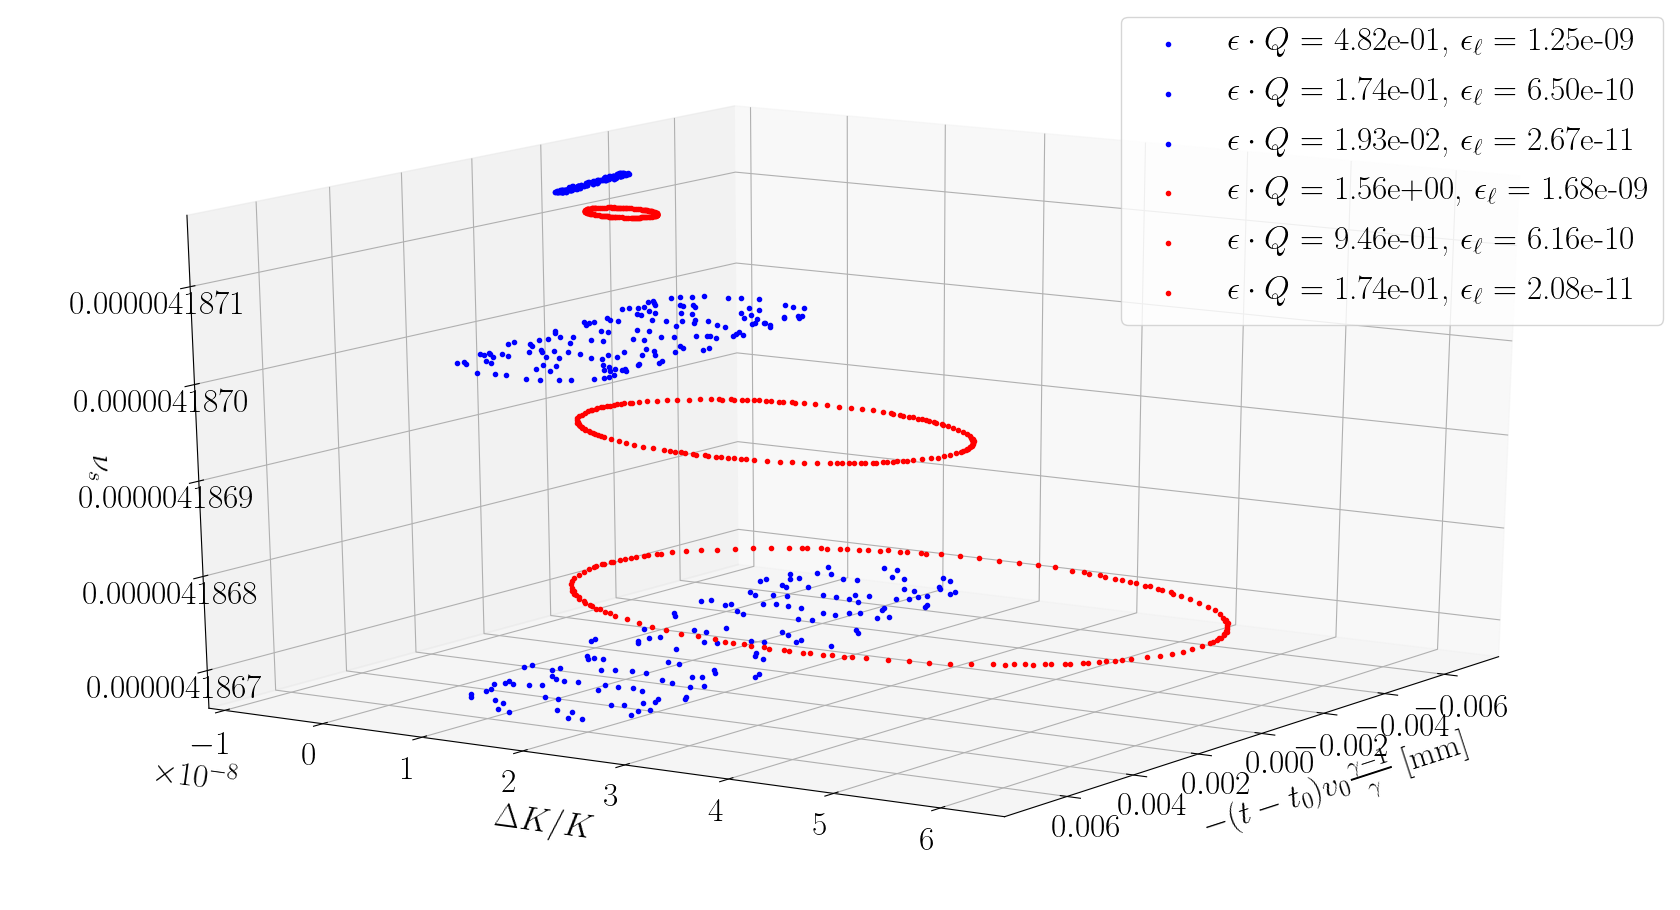
\includegraphics[width=.9\linewidth,
			trim=45 0 0 0, clip]{stune_traj_equ/part2/3D_plot_all_ps_vars_equal_long_emi}};
	\end{tikzpicture}
\end{frame}
\begin{frame}{Conclusions}
	\begin{block}{Conclusion 1}
	\begin{itemize}
		\item Spin tune is reducible to a univariate function
		\item Effective Lorentz-factor is a measure of the particle's longitudinal emittance
	\end{itemize}
	\end{block}
\end{frame}
\begin{frame}{Conclusions}\centering
	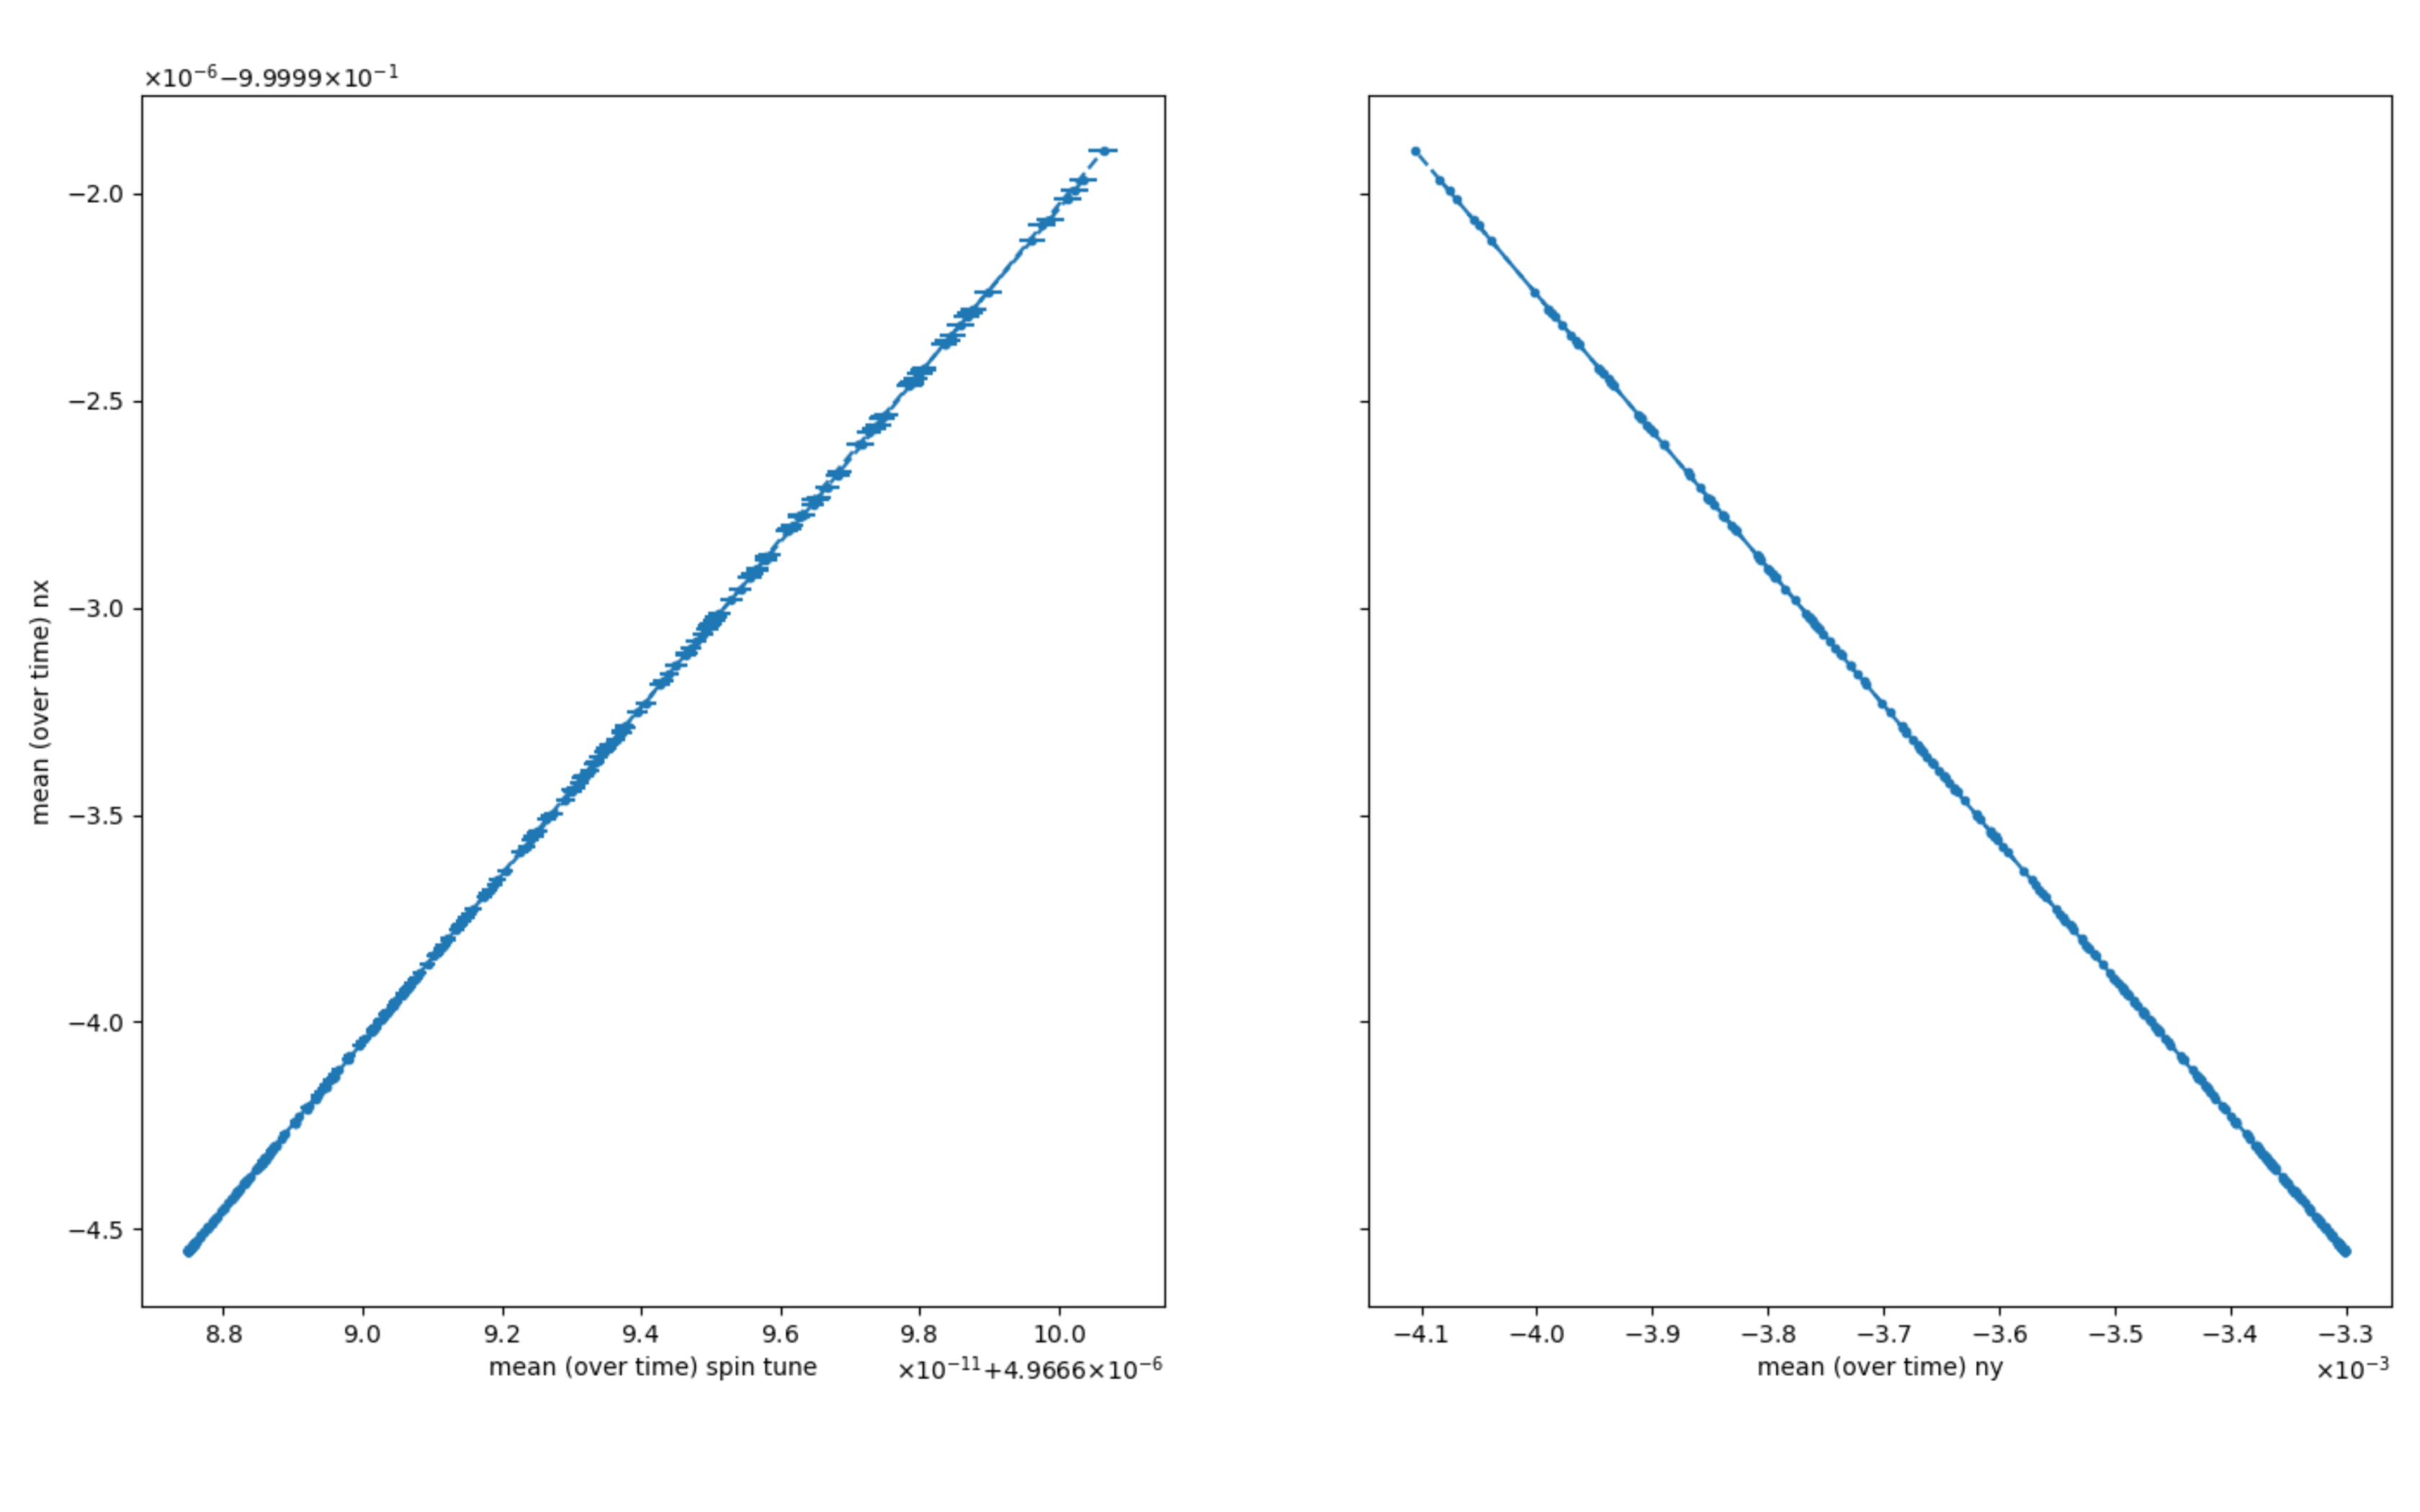
\includegraphics[width=.9\linewidth]{decoh_sim/mean_n_bar_vs_spin_tune}
\end{frame}
\begin{frame}{Conclusions}
	\begin{block}{Conclusion 2}
		The spin dynamics of particles with the same value of $\gef$ are equivalent in the gerenal sense ($\nu_s$, $\nbar$)
	\end{block}
	\pause
	\begin{alertblock}{Disclaimer}
		At least for the Frozen Spin lattice that I used in simulations
	\end{alertblock}
\end{frame}

\end{document}